\chapter{Diffusion Limit Results}
\label{Diffusion Limit Results}

The following chapter approaches the issue of complexity of Metropolis-Hastings~(MH) methods for a class of target distributions obtained by a change of measure from a Gaussian measure on an infinite dimensional Hilbert space. This Hilbert setting is widely used in applications as diffusion bridges and Bayesian inverse problems, see Chapter~\ref{Application}. Mattingly, Pillai and Stuart~\autocite{Mattingly2010} and Pillai, Stuart and Thi\'{e}ry~\autocite{Pillai2012} proved that under certain conditions on the regularity of the change of measure and the decay of eigenvalues of the Gaussian covariance operator, a diffusion limit process exists for a suitable scaled version of the MH Markov chain. Hence, according to the research programm initiated by Roberts and coworkers in the pair of papers~\autocite{Roberts1997, Roberts1998} and presented in Chapter~\ref{CC:Optimality and Diffusion Limits}, a computational complexity of $\mathcal{O}(N)$ for the Random Walk Metropolis~(RWM) (introduced in Chapter~\ref{MH-RWM}) and of $\mathcal{O}(N^{1/3})$ for the Metropolis Adjusted Langevin Algorithm~(MALA) (introduced in Chapter~\ref{MH-MALA}) is achieved with dimension~$N$ going to infinity.

This elaboration follows the structure of the the two main references of Mattingly, Pillai and Stuart~\autocite{Mattingly2010} and Pillai, Stuart and Thi\'{e}ry~\autocite{Pillai2012}. Most statements and proofs are taken from these two papers. Since it is our goal to point out a common structure in this two proofs to restate the two main diffusion limit results as one theorem, we will refer to the original papers~\autocite{Mattingly2010, Pillai2012} for several technical estimates.

In Chapter~\ref{sec:DLR-Preliminaries} we define precisely the setting in which the diffusion limit result holds. In Chapter~\ref{sec:DLR-Main theorem} we state the main theorem for RWM and MALA simultaneously and explain it. Chapter~\ref{sec:DLR-Proof} contains the proof of the main theorem, postponing the proof of a number of key technical estimates to Chapter~\ref{sec:DLR-Estimates}.


\subsubsection{Motivation}

We have seen that in applications such as Bayesian approach to inverse problems and conditioned diffusions (see Chapter~\ref{Application}), the target measure of interest, $\pi$, is defined on an infinite dimensional real separable Hilbert space~$\mathcal{H}$. In the case of Gaussian priors (inverse problems) or additive noise (diffusions), $\pi$ is absolutely continuous with respect to a Gaussian reference measur~$\pi_0$ on $\mathcal{H}$ with mean zero and covariance operator~$\mathcal{C}$. The Radon-Nikodym derivative is assumed to have the form
\begin{equation}
\label{DLR-Radon Nikodym derivative}
 \frac{d \pi}{d \pi_0}(x) = M_{\Psi} \exp (- \Psi(x))
\end{equation}
for a real-valued $\pi_0$-measurable functional~$\Psi$ on the Hilbert space and $M_{\Psi}$ is a normalizing constant. This infinite dimensional framework for target measures~$\pi$ of the form~(\ref{DLR-Radon Nikodym derivative}) introduces an inherent mathematical structure which make it conceivable to derive a diffusion limit result for this class of target measures. We highlight two aspects of this mathematical structure. 

First, the theory of Gaussian measures on infinite dimensional Hilbert spaces~$\mathcal{H}$ introduces with the covariance operator~$\mathcal{C}$ the possibility to represent $\mathcal{H}$ via an orthonormal basis of eigenvectors of the $\mathcal{C}$. This representation combined with the Karhunen-Lo\`{e}ve expansion allows us to express any element of~$\mathcal{H}$ distributed according to the reference measure~$\pi_0$ as a possible infinite sum of independent Gaussian random variables. Under certain regularity conditions on~$\Psi$, this subtle product structure is transfered to the target measure corresponding to the change of measure represented by~$\Psi$. This Gaussian embedding is the is the main reason for the working approximation estimates in Chapter~\ref{sec:DLR-Estimates}.

The second aspect of this inherent mathematical structure is the existence of a putative limit diffusion process. In order to prove a limit result as desired, a diffusion candidate is needed, i.e. a diffusion process which is invariant with respect to~$\pi$. In the abstract infinite dimensional Hilbert space setting, linear stochastic partial differential equations~(SPDE) are well understood, e.g. \autocite{DaPrato1992, Hairer2005, Hairer2007}. In the case of linear SPDEs  of the form
\begin{equation}
 dx =  \mathcal{A} x dt + \sqrt{2} \, d \mathcal{W}(t) \qquad x(0)  =0,
\end{equation}
where $ \mathcal{W}(t) $ is a cylindrical Wiener process in $\mathcal{H}$ and $\mathcal{A}$ a suitable linear operator on~$\mathcal{H}$, the invariant distribution is the Gaussian measure~$ \nu = \mathcal{N}(0, -\mathcal{A}^{-1})$ on $\mathcal{H}$. As usual in the theory of (S)PDEs, the linear case is a jumping-off point to the nonlinear equations, just as in this situation. The preconditioned semilinear SPDE is of the form
\begin{equation}
\label{DLR- preconditioned semilinear SPDE - langevin}
 dx = \mathcal{G} (\mathcal{A}x + F(x))dt + \sqrt{2}\mathcal{G}^{1/2} d\mathcal{W}(t), \qquad x(0) = x_0,
\end{equation}
where $\mathcal{A}$ and $\mathcal{W}(t)$ as above and $F: \mathcal{H} \to \mathcal{H}$ is a Fr\'{e}chet differentiable nonlinearity or drift and $\mathcal{G}$ is a self-adjoint, positive linear operator on $\mathcal{H}$, the so-called preconditioner; for further details, we refer to \autocite{Hairer2005, Hairer2007}. These type of SPDE may be viewed as an infinite dimensional analogue of the Langevin equation used in finite dimensions. Accordingly, we will call these SPDEs given by Equation~(\ref{DLR- preconditioned semilinear SPDE - langevin}) \textit{Langevin equations}. Under the assumption that $F = \nabla U$ for a  Fr\'{e}chet differentiable function $U: \mathcal{H} \to \mathbb{R}$ and some regularity conditions on the linear operators~$\mathcal{A}$ and $\mathcal{G}$, the invariant distribution for the Langevin equation defined in Equation~(\ref{DLR- preconditioned semilinear SPDE - langevin}) is given by 
\begin{equation}
 d \eta (x) = M \, e^{U(x)} \, d \nu (x)
\end{equation}
with $\nu = \mathcal{N}(0, - \mathcal{A}^{-1})$. Taking $U = - \Psi$, $\mathcal{G}= \mathcal{C}$ and $\mathcal{A}= - \mathcal{C}^{-1}$, which is well-defined in the case of $\mathcal{C}$ being a covariance operator as considered above, we obtain a $ \mathcal{H} $-valued SDE with the form
\begin{equation}
\label{DLR-limit diffusion candidate}
 dz = - ( z + \mathcal{C} \nabla \Psi (z) ) dt + \sqrt{2} \mathcal{C}^{1/2} d \mathcal{W}(t), \quad z(0) = z_0,
\end{equation}
where $ \mathcal{W}(t) $ is a cylindrical Wiener process in $\mathcal{H}$ and the invariant measure is of the form of $\pi$ as given in Equation~(\ref{DLR-Radon Nikodym derivative}). Moreover, it is shown~\autocite[Theorem 3.6]{Hairer2007}, that Equation~(\ref{DLR- preconditioned semilinear SPDE - langevin}) has a unique strong and continuous solution. Thus, we have a natural candidate for the infinite dimensional limit diffusion process.
\newline

In this setup, our perspective is to apply MCMC methods to finite approximations of the measure~$\pi$ found by projecting onto the first $N$ eigenfunctions of the covariance operator~$\mathcal{C}$ of the Gaussian reference measure~$\pi_0$. These projections allow us to hope for a consistent definition of the finite dimensional approximations. In the following section, we will define this setting rigorously such that we can define the RWM- and MALA-type algorithms and we state the diffusion limit result precisely.


\section{Hilbert Space Setting, Assumptions, Projections - Preliminaries}
\label{sec:DLR-Preliminaries}

This section is devoted to stating the setting of the main theorem. As suggested in Chapter~\ref{Application}, the considered setting is complex, and we develop it in a step-by-step fashion. We first introduce the Gaussian reference measure~$\pi_0$ and the change of measure which induces a genuinely nonproduct structure. We then describe a finite dimensional approximation of the measure, enabling us to define a RWM- and MALA-type algorithm.

The structure and most definitions are taken from~\autocite[Section 2]{Pillai2012}. At some passages, we amended it. References for this additonal work will be explicitely given in the text.

\subsubsection{Gaussian Reference Measure}

Let $\mathcal{H}$ be a separable Hilbert space of real-valued functions with inner-product denoted by $\langle \cdot, \cdot \rangle$ and associated norm $\|x\|^2 = \langle x, x \rangle$. Consider a (non-degenrated) Gaussian measure~$\pi_0$ on $(\mathcal{H}, \|\cdot\|)$ with covariance operator~$\mathcal{C}$. According to the general theory of Gaussian measures~\autocite[Chapter I]{DaPrato1992}, $\mathcal{C}$ is a self-adjoint and positive trace class operator on $\mathcal{H}$. Although the concept of Gaussian measures on (infinite dimensional) Hilbert spaces should be familiar to the reader, we briefly recall the definitions of the mean and the covariance of Gaussian measures in Hilbert spaces and the definition of \textit{trace class} operators, since this point is crucial for the understanding.

We start with the definition of Gaussian measures on Hilbert spaces, taken from~\autocite[Section 2.3.2]{DaPrato1992}.

\begin{defin}
\label{DLR-Setting: Definition Gaussian measure}
 Let $(\mathcal{H}, \|\cdot\|)$ be a Hilbert space with inner-product denoted by $\langle \cdot, \cdot \rangle$, a probabiity measure~$\mu$ on $\mathcal{H}$ is called Gaussian if for arbitrary $y \in \mathcal{H}$ there exist $a \in \mathbb{R}^1, q \geq 0$, such that,
 \begin{equation*}
  \mu \{ x \in \mathcal{H}: \langle y, x \rangle \in D \} = \mathcal{N}(a, q) (D), \qquad D \in \mathcal{B}(\mathbb{R}^1).
 \end{equation*}
\end{defin}

 In particular, if $\mu$ is Gaussian, then there exist an element $m \in \mathcal{H}$ and a self-adjoint, positive and continuous operator $\mathcal{C}$ such that:
 \begin{align}
  \int_{\mathcal{H}} \langle y, x \rangle \mu (dx) = \langle m, y \rangle, \qquad \forall y \in \mathcal{H}, \\
  \int_{\mathcal{H}} \langle y, x - m \rangle \langle z, x - m \rangle \mu (dx) = \langle \mathcal{C}y, z \rangle, \qquad \forall y, z \in \mathcal{H}.
 \end{align}
The element $m \in \mathcal{H}$ is called the \textit{mean} and $\mathcal{C}$ the \textit{covariance} operator of $\mu$. Moreover, the characteristic function of $\mu$ is given by 
\begin{equation*}
 \widehat{\mu} (h) := \int_{\mathcal{H}} e^{i \langle h, x \rangle} \mu(dx) = e^{i \langle h, m \rangle - \tfrac{1}{2} \langle \mathcal{C} h, h \rangle}, \qquad h \in \mathcal{H}.
\end{equation*}
It is therefore uniquely determined by $m$ and $\mathcal{C}$ and is denoted by $ \mathcal{N}(m, \mathcal{C})$.

The covariance operator~$\mathcal{C}$ has some further properties, it turns out that it is a trace class operator~\autocite[Proposition 2.15]{DaPrato1992}.

\begin{defin}\autocite[Section 1.1]{DaPrato2002}
\label{DLR-Setting: Definition trace class}
 Let $\mathcal{H}$ be a separable Hilbert space with inner-product and norm denoted by $\langle \cdot, \cdot \rangle$ and $\| \cdot \|$. A bounded linear operator $\mathcal{A}$ on $\mathcal{H}$ is said to be of trace class if there exist two sequences~$\{ a_j \}, \{ b_j \}$ in $\mathcal{H}$ such that
 \begin{equation*}
  \mathcal{A}x := \sum_{j \in I} \langle x, a_j \rangle b_j, \qquad x \in \mathcal{H},
 \end{equation*}
 and
 \begin{equation*}
  \sum_{j \in I} \| a_j \| \| b_j \| < + \infty.
 \end{equation*}
 If an operator~$\mathcal{A}$ is of trace class then its trace, $\text{Tr}_{\mathcal{H}}\mathcal{A}$, is defined by the formula
 \begin{equation}
  \text{Tr}_{\mathcal{H}}(\mathcal{A}) := \sum_{j \in I} \langle e_j, \mathcal{A} e_j \rangle,
 \end{equation}
 where~$\{ e_j : j \in I \}$  is an orthonormal and complete basis on $\mathcal{H}$.

\end{defin}

Trace class operators have some usefull properties. First, note that the definition of the trace is independent of the orthonormal basis~\autocite[Proposition C.1]{DaPrato1992}. More important is the following fact: if $\mathcal{A}$ is a positive and self-adjoint trace class operator (like the covariance operator~$\mathcal{C}$) then it is diagonizable (being a bounded trace class operator implies that it is compact): there is an orthonormal basis~$\{ e_j : j \in I \}$ for $\mathcal{H}$ consisting of eigenvectors of $\mathcal{A}$ such that $\mathcal{A} e_j = \eta_j e_j $ and $\eta_j > 0, \sum_{j \in I} \eta_j < + \infty$; see~\autocite[Lemma 6.32]{Dashti2014} and~\autocite[Proposition 3.15]{Hairer2009}. Thus, a given Gaussian measure introduces a lot of structure in form of a complete eigenbasis to the underlying Hilbert space. This subtle structure is essential in the proof of the diffusion limit result.


Therefore, let $\{ \varphi_j, \lambda_j^2 \}_{j \geq 1}$ be the eigenfunctions and eigenvalues of the covariance operator~$\mathcal{C}$ of the Gaussian measure~$\pi_0$:
\begin{equation}
\label{DLR-Setting: Eigefunctions}
 \mathcal{C} \varphi_j = \lambda_j^2 \varphi_j, \qquad j \geq 1. 
\end{equation}
We assume a normalization under which $\{ \varphi_j \}_{j \geq 1}$ forms a complete orthonormal basis in the Hilbert space $\mathcal{H}$, which we refer to us as the Karhunen-Lo\`{e}ve basis. Henceforth, we assume that the eigenvalues are arranged in decreasing order and note $\lambda_j > 0$. Any function~$x \in \mathcal{H}$ can be represented in the orthonormal eigenbasis of $\mathcal{C}$ via the expansion
\begin{equation}
\label{DLR-Setting: karhunen-loeve representation}
 x = \sum_{j = 0}^{\infty} x_j \varphi_j, \qquad x_j := \langle x, \varphi_j \rangle.
\end{equation}
It will often be helpfull, to identify the function~$x$ with its coordinates~$\{ x_j \}_{j=1}^{\infty} \in l^2$ in the eigenbasis and vice versa, where $l^2$ denotes the sequence space of square summable sequences. By the Karhunen-L\`{e}ve or white noise expansion~\autocite[Section 2.2.3]{DaPrato1992}, a realization~$x$ from the Gaussian reference measure~$\pi_0$ can be expressed by allowing the coordinates~$\{x_j\}_{j \geq 1}$ to be independent Gaussian random variables distributed according $\mathcal{N}(0, \lambda_j^2)$ in $\mathbb{R}$. Thus, the Gaussian reference measure~$\pi_0$ has a product structure in the coordinate-representation.
\newline


Frequently in applications, the functional~$\Psi$ in Equation~(\ref{DLR-Radon Nikodym derivative}) may not be well-defined on all of $\mathcal{H}$, in the sense that some regularity conditions on $\Psi$ hold only on a subset $\mathcal{H}^r \subset \mathcal{H}$ for some exponent~$r > 0$. For instance, if $ \mathcal{H}= L^2([0,1]) $, the functional~$\Psi$ might only act on continuous functions well, in which case it is natural to define~$\Psi$ on some Sobolev-like space~$\mathcal{H}^r([0,1])$ for $r > \tfrac{1}{2}$. There exist Sobolev embeddings for such Sobolev-like spaces~$\mathcal{H}^r$, which we will define now~\autocite[Theorem 6.3]{Hairer2009}.


To follow this purpose, we now think of Sobolev-like spaces~$\mathcal{H}^r , r \in \mathbb{R}$, also called Hilbert scale spaces. Given a Hilbert space~$ (\mathcal{H}, \langle \cdot, \cdot \rangle, \| \cdot \|) $ of real-valued functions, and  $\{ \varphi_j \}_{j \geq 1}$ an orthonormal basis for~$\mathcal{H}$, for any $x \in \mathcal{H}$ the representation in Equation~(\ref{DLR-Setting: karhunen-loeve representation}) holds. Thus, we can define
\begin{equation}
 \mathcal{H}^r := \left\{ x \in \mathcal{H}: \| x \|_r^2 < \infty \right\}
\end{equation}
where $r \in \mathbb{R}$ and, for $ x_j = \langle x, \varphi_j \rangle $,
\begin{equation}
\label{DLR-Setting: H^r norm}
 \| x \|_r^2 := \sum_{j=1}^{\infty} j^{2r} x_j^2.
\end{equation}
In fact $\mathcal{H}^r$ is a Hilbert space: for $ y_j = \langle y, \varphi_j \rangle $ we define the inner-product
\begin{equation}
 \langle x, y \rangle_{r} := \sum_{j=1}^{\infty} j^{2r} x_j y_j.
\end{equation}
For any $r>0$, the Hilbert space~$ (\mathcal{H}^r, \langle \cdot, \cdot \rangle_r, \| \cdot \|_r) $ is a subset of the original Hilbert space~$\mathcal{H}$; for $r<0$ the spaces are defined by duality and are supersets of $\mathcal{H}$. These spaces are again separable Hilbert spaces for any $r \in \mathbb{R}$ as they are linked to the sequence space~$l^2$ with weights~$\omega_j = j^{2r}$ which are separable~\autocite[Section 6.1.3]{Dashti2014}.

For $x,y \in \mathcal{H}^r$, the outer product operator in $\mathcal{H}^r$ is the operator~$ x \otimes_{\mathcal{H}^r} y : \mathcal{H}^r \to \mathcal{H}^r $ defined by $ (x \otimes_{\mathcal{H}^r} y) z := \langle y, z \rangle_r x $ for every $ z \in \mathcal{H}^r$. Moreover, we want to transfer the covariance operator~$\mathcal{C}$ to $\mathcal{H}^r$. For $r \in \mathbb{R}$, let $B_r: \mathcal{H} \to \mathcal{H}$ denote the operator which is diagonal in the basis~$\{ \varphi_j \}_{j \geq 1}$ with diagonal entries~$j^{2r}$ so that $B_r^{1/2} \varphi_j = j^{r} \varphi_j$. The operator~$B_r$ lets us alternate between $\mathcal{H}$ and $\mathcal{H}^r$ by the following identity $ \langle x, y \rangle_r = \langle B_r^{1/2} x, B_r^{1/2} y \rangle$. Since $B_r^{-1/2} $ is an isometry, the family~$\{ \phi_j \}_{j \geq 1}$ forms a complete orthonormal basis for~$\mathcal{H}^r$ with $ \phi_j(r) := B_r^{-1/2} \varphi_j$. Similar to Definition~\ref{DLR-Setting: Definition trace class}, we can define the trace on $\mathcal{H}^r$ by
\begin{equation}
 \label{DLR-Setting: Trace on H^s}
 \text{Tr}_{\mathcal{H}^r}(\mathcal{A}) := \sum_{j=1}^{\infty} \langle (B_r^{-1/2}\varphi_j ), \mathcal{A}( B_r^{-1/2}\varphi_j) \rangle_r.
\end{equation}
For a positive and bounded operator~$\mathcal{A}$ it suffices to show that the trace~$\text{Tr}_{\mathcal{H}^r}(\mathcal{A})$ is finite, to conclude that $\mathcal{A}$ is of trace class~\autocite[Proposition C.3]{DaPrato1992}. We define the linear operator~$\mathcal{C}_r := B_r^{1/2} \mathcal{C} B_r^{1/2} $ with $ \text{Tr}_{\mathcal{H}^r}(\mathcal{C}_r) = \sum_{j=0}^{\infty} \lambda_j^2 j^{2r}$. Under the condition
\begin{equation}
\label{DLR-Setting: Gaussian measure on H^r condition}
 \text{Tr}_{\mathcal{H}^r}(\mathcal{C}_r) < \infty,
\end{equation}
we can conclude that the positive and self-adjoint operator~$\mathcal{C}_r$ is of trace class and therefore it exists a Gaussian measure on~$\mathcal{H}^r$ with covariance operator~$\mathcal{C}_r$~\autocite[Proposition 2.18]{DaPrato1992}. This Gaussian measure on~$\mathcal{H}^r$ is induced by the reference measure~$\pi_0$ on~$\mathcal{H}$, and $ \pi_0(\mathcal{H}^r ) =1$, if the condition in Equation~(\ref{DLR-Setting: Gaussian measure on H^r condition}) holds. Indeed, we claim that $\mathcal{C}_r$ is the covariance operator of the Gaussian measure~$\pi_0$ on $\mathcal{H}^r$ by verifying the definitions; see~\autocite[Chapter 2.3]{DaPrato1992} for an introduction to Gaussian measures on Hilbert spaces.

\begin{proposition}
\label{DLR-Setting: Proposition Gaussian measure}
 Let $\xi \stackrel{D}{\sim} \pi_0$, then $\mathbb{E} [\langle \xi, u \rangle_r \langle \xi , v \rangle_r ] = \langle u , \mathcal{C}_r v \rangle_r$ for any functions $u,v \in \mathcal{H}^r$. Similarly, $\mathbb{E} [\langle \xi, u \rangle_r  ] = 0$ for any function $u \in \mathcal{H}^r$.
\end{proposition}

\begin{proof}
 Let $\xi \stackrel{D}{\sim} \pi_0$, then by using the definition of the covariance operator~$\mathcal{C}$ and of the inner-product $\langle \cdot, \cdot \rangle_r$, we conclude,
 \begin{align*}
  \int_{\mathcal{H}} \langle \xi, u \rangle_r \langle \xi , v \rangle_r \; \pi_0 (d\xi) & \; = \langle \mathcal{C} B_r u , B_r v \rangle \\
  & \; = \langle B_r^{1/2} \mathcal{C} B_r u , B_r^{1/2} v \rangle \\
  & \; = \langle  B_r u , \mathcal{C}_r v \rangle \\	
  & \; = \langle  B_r^{1/2} u , B_r^{1/2} \mathcal{C}_r v \rangle = \langle u, \mathcal{C}_r v \rangle_r.
 \end{align*}
 We used the self-adjointness of $\mathcal{C}$ and $B_r$. Similarly, we can conclude for the mean.

\end{proof}

Additionally, we claim that if $\text{Tr}_{\mathcal{H}^r}(\mathcal{C}_r)$ is finite, $\pi_0$ has full support on the subspace $\mathcal{H}^r$.

\begin{proposition}
\label{DLR-Setting: Proposition Full support}
 Under the condtion given in Equation~(\ref{DLR-Setting: Gaussian measure on H^r condition}), $\pi_0 $-almost every function~$x \in \mathcal{H}$ belongs to $\mathcal{H}^r$.
\end{proposition}

\begin{proof}
 Let $x \in \mathcal{H}$, then by monotone convergence and using the definition of the covariance operator~$\mathcal{C}$ of the Gaussian measure~$\pi_0$, we conclude
 \begin{align*}
  \int_{\mathcal{H}} \| x \|_r^2 \; \pi_0 (dx) & \; = \int_{\mathcal{H}} \sum_{j=1}^{\infty} x_j j^{2r} \; \pi_0 (dx)  \\
  & \; = \sum_{j=1}^{\infty} j^{2r} ( \int_{\mathcal{H}}  \langle x, \varphi_j \rangle^2  \; \pi_0 (dx) )  \\
  & \; = \sum_{j=1}^{\infty} j^{2r} (   \langle \mathcal{C} \varphi_j, \varphi_j \rangle   )    \\
  & \; = \sum_{j=1}^{\infty} j^{2r} \lambda_j^2 < \infty.
 \end{align*}
 The first and second identy follows from the representation of the $\mathcal{H}^r$-norm in Equation~(\ref{DLR-Setting: H^r norm}) and the Karhunen-Lo\'{e}ve representation in Equation~(\ref{DLR-Setting: karhunen-loeve representation}). As $\{  \varphi_j \}_{j \geq 1}$ are eigenfunctions of $\mathcal{C}$ as stated in Equation~(\ref{DLR-Setting: Eigefunctions}) and $\text{Tr}_{\mathcal{H}^r}(\mathcal{C}_r) < \infty$ as assumed, we finish the proof.

\end{proof}

Hence, we alternate between both Gaussian measures~$\mathcal{N}(0, \mathcal{C})$ on $\mathcal{H}$ and $\mathcal{N}(0, \mathcal{C}_r)$ on $\mathcal{H}^r$, for those $r$ for which $\text{Tr}_{\mathcal{H}^r}(\mathcal{C}_r)$ is finite. Moreover, there will be a subtle change in the choice of the basis. In the next subsection we will fix an exponent~$r>0$ and denote it by~$s$ such that $\text{Tr}_{\mathcal{H}^s}(\mathcal{C}_s) < \infty$. By doing this, we will completely switch to this Sobolev space~$\mathcal{H}^s$, in particular we will considering the basis~$\phi_j(s) = \phi_j := B^{-1/2}_s \varphi_j$. Thus, every coordinate of an object of~$\mathcal{H}^s$ will be given with respect to this basis. To avoid irritation, we recall some definitions and facts due to this basis change. The inner product on $\mathcal{H}^s$ reads
\begin{equation}
  \langle x, y \rangle_s = \sum_{j=1}^{\infty} x_j y_j \quad \text{ for } x_j = \langle x, \phi_j\rangle_s
\end{equation}
and the norm on $\mathcal{H}^s$ is given by
\begin{equation}
  \| x \|_s^2 = \sum_{j=1}^{\infty} x_j^2 \quad \text{ for } x_j = \langle x, \phi_j\rangle_s.
\end{equation}
On $\mathcal{H}^s$ we will consider the positive, self-adjoint trace-class operator~$\mathcal{C}_s$ with the eigenbasis~$\{ \phi_j,  \lambda_j^2 j^{2s} \}_{j \geq 1}$ of the Gaussian measure~$\pi_0$ projected to $\mathcal{H}^s$: for $j \geq 1$
\begin{equation}
\label{DLR-Setting: Definition Eigefunctions of C_s}
   \mathcal{C}_s \phi_j = B_s^{1/2} \mathcal{C}B^{1/2}_sB^{-1/2}_s \varphi_j  =  \lambda_j^2 j^s \varphi_j = ( \lambda_j^2 j^{2s}) \phi_j.
\end{equation}

\begin{rem}
  In comparison to~\autocite{Mattingly2010, Pillai2012}, we change the notation as we will consequently use the eigenbasis~$\{ \phi_j,  \lambda_j^2 j^{2s} \}_{j \geq 1}$ of $\mathcal{C}_s$ on $\mathcal{H}^s$. This basis change do not disrupt the results given in the original papers but it allows us to work with the operator~$\mathcal{C}_s$ instead of $\mathcal{C}$ such that we can state our main result in a consitent fashion. As we will refer to these original works for some  proofs, we want to emphasize that all calculations with the operator~$\mathcal{C}$ in its eigenbasis~$\{ \varphi_j,  \lambda_j^2 \}_{j \geq 1}$ do not change if one considers the operator~$\mathcal{C}_s$ with its eigenbasis~$\{ \phi_j,  \lambda_j^2 j^{2s} \}_{j \geq 1}$ instead. Indeed, we have
  \begin{equation}
    \begin{split}
      \| \mathcal{C}x \|_s^2 & = \sum_{j=1}^{\infty} j^{2s} \lambda_j^2 \left(x_j^2 (\mathcal{H})\right), \\
       \| \mathcal{C}_sx \|_s^2 & = \sum_{j=1}^{\infty} j^{2s} \lambda_j^2 \left(x_j^2(\mathcal{H}^s)\right),\\
    \end{split}
  \end{equation}
 where we distinguished between the two coordinates~$x_j^2 (\mathcal{H}) $ with respect to the eigenbasis of~$\mathcal{C}$ and $x_j^2(\mathcal{H}^s)$ with respect to the eigenbasis of $\mathcal{C}_s$.
\end{rem}




\subsubsection{Change of Measure}

The target measure of interest, $\pi$, from which we want to sample is defined through the change of measure defined in Equation~(\ref{DLR-Radon Nikodym derivative}) via the functional~$\Psi$. As the measure~$\pi_0$ has full support on~$\mathcal{H}^s$, if $\text{Tr}_{\mathcal{H}^r}(\mathcal{C}_r) < \infty$, the functional~$\Psi$ needs only to be defined on $\mathcal{H}^s$ such that the Radon-Nikodym derivative of the change of measure is well-defined.

We will give assumptions on the decay of eigenvalues of the covariance operator~$\mathcal{C}$ of~$\pi_0$ in order to ensure the existence of a real number~$s > 0$ such that Equation~(\ref{DLR-Setting: Gaussian measure on H^r condition}) is fulfilled and $\pi_0$ has full support on $\mathcal{H}^s$. Furthermore, we impose regularity conditions on the functional~$\Psi$. These assumptions shall ensure that the target measure~$\pi$ is not too different from the Gaussian measure~$\pi_0$ such that we can ascribe further properties of the Gaussian measure~$\pi_0$ to $\pi$~(see Lemma~\ref{} and Lemma~\ref{}). These assumptions can be summarized in the following way: the functional~$\Psi$ has to be quadratically bounded, with first derivative linearly bounded, and the second derivative globally bounded. By using the identification of the dual spaces for Hilbert spaces, we can formulate our assumptions precisely, see~\autocite[Assumption 2.1]{Pillai2012} for further details.

\begin{assum}
 \label{DLR-Setting: Assumptions on C and Psi}
 The covariance operator $\mathcal{C}$ and the functional~$\Psi$ satisfy the following:
 \begin{enumerate} 
  \item[(1)] \textit{Decay of Eigenvalues~$\lambda_j^2$ of $\mathcal{C}$: } There is an exponent~$\kappa > \tfrac{1}{2}$ such that
 \begin{equation}
 \label{DLR-Seeting: Assumption on decay of eigenvalues}
  \lambda_j \asymp j^{- \kappa}.
 \end{equation}
 \item[(2)] \textit{Assumptions on $\Psi$: } There exist constants $M_i \in \mathbb{R}, i \leq 4$, and $s \in [0, \kappa - 1/2)$ such that for all $x \in \mathcal{H}^s$ the functional~$\Psi: \mathcal{H}^s \to \mathbb{R}$ satisfies
 \begin{align}
 \label{DLR-Setting: Assumption on Psi 1}
  M_1 & \; \leq \Psi(x) \leq M_2 (1+ \| x \|_s^2), \\
  \label{DLR-Setting: Assumption on Psi 2}
  \| \nabla \Psi (x) \|_{-s} & \; \leq M_3 (1+\| x\|_s), \\
  \label{DLR-Setting: Assumption on Psi 3}
  \| \partial^2 \Psi (x) \|_{\mathcal{L}(\mathcal{H}^s, \mathcal{H}^{-s})} & \; \leq M_4.
 \end{align}
 \end{enumerate}
\end{assum}

Here we used the following notation. Two sequences $\{\alpha_n\}$ and $\{\beta_n\}$ satisfy $\alpha_n \lesssim  \beta_n$ if there exists a constant~$M>0$ such that $\alpha_n \leq M \; \beta_n$ for all $n \leq 0$. The notation~$\alpha_n \asymp \beta_n$ means that $\alpha_n \lesssim  \beta_n $ and $ \beta_n \lesssim  \alpha_n$~\autocite{Pillai2012}.

\begin{rem}
 The growth condition~$\kappa > \tfrac{1}{2}$ ensures that the covariance operator~$\mathcal{C}$ of~$\pi_0$ is of trace class as $\text{Tr}_{\mathcal{H}}(\mathcal{C}) = \sum_{j=1}^{\infty} \lambda_j^2$. In fact, the condition on the trace of~$\mathcal{C}_r$ in Equation~(\ref{DLR-Setting: Gaussian measure on H^r condition}) is satistied if and only if $r < \kappa - \tfrac{1}{2}$. Indeed, under Assumption~\ref{DLR-Setting: Assumptions on C and Psi}, we calculate
 \begin{equation*}
  \text{Tr}_{\mathcal{H}^r}(\mathcal{C}_r) = \sum_{j=1}^{\infty} \lambda_j^2 j^{2r}  \asymp \sum_{j=1}^{\infty} j^{2(r-\kappa)} < \infty, \qquad \text{for } \; r < \kappa - \tfrac{1}{2}.
 \end{equation*}
 We choose now and for the rest of this chapter, $s \in [0, \kappa - \tfrac{1}{2})$. We define the Sobolev space~$\mathcal{H}^s$ and the reference Gaussian measure~$\pi_0$ has full support on~$\mathcal{H}^s$ as the condition in Equation~(\ref{DLR-Setting: Gaussian measure on H^r condition}) is fulfilled. Thus, the Radon-Nikodym derivative of $\pi$ in Equation~(\ref{DLR-Radon Nikodym derivative}) is well-defined with the change of measure~$\Psi$. Indeed, all regularity assumptions on~$\Psi$ given in Assumption~\ref{DLR-Setting: Assumptions on C and Psi} are defined on $\mathcal{H}^s$ a subset of $\mathcal{H}$ with full measure under~$\pi_0$. These assumptions ensure $\Psi$ to be Lipschitz-continuous on $\mathcal{H}^s$ and therefore it is $\pi_0$-measurable. 

\end{rem}


\begin{rem}
  The assumption on the decay of eigenvalues~$\lambda_j^2$ of $\mathcal{C}$ results directly in the decay of eigenvalues~$\lambda_j^2 j^{2s}$ of $\mathcal{C}_s$: There is an exponent~$\kappa > \tfrac{1}{2}$ such that
 \begin{equation}
 \label{DLR-Seeting: Assumption on decay of eigenvalues of C_s}
 \lambda_j j^{s} \asymp j^{s - \kappa}.
 \end{equation}
 As $s < \kappa -\tfrac{1}{2}$, we conclude: $ s -\kappa < - \tfrac{1}{2} $.
\end{rem}



The assumptions given on the decay of eigenvalues of $\mathcal{C}$ given in Equation~(\ref{DLR-Seeting: Assumption on decay of eigenvalues}) implies that the covariance operator~$\mathcal{C}_s$ has a smoothing effect.

\begin{lemma}\autocite[Lemma 3.3]{Mattingly2010}
\label{DLR-Setting: Smoothing effect of C}
 Under Assumption~\ref{DLR-Setting: Assumptions on C and Psi}, it follows that for all~$\alpha \in \mathbb{R}$,
 \begin{equation}
   \| \mathcal{C}_s^{\alpha} x \|_{s} \asymp \| x \|_{2 \alpha (s - \kappa)}, \qquad \text{for } x \in \mathcal{H}^s.
 \end{equation}
 
\end{lemma}

\begin{proof}
 By using the decay of eigenvalues of~$\mathcal{C}_s$, we establish both required inequalities from the definitions of the appropriate norms.
 \begin{equation*}
   \| \mathcal{C}_s^{\alpha} x \|_{s}^2 = \sum_{j=1}^{\infty} (j^{2 s} \lambda_j^2)^{2 \alpha} x_j^2 \asymp  \sum_{j=1}^{\infty} j^{4 \alpha (s - \kappa)} x_j^2 = \| x \|_{ 2 \alpha ( s - \kappa)}^2.
 \end{equation*}

\end{proof}


\subsubsection{Finite Dimensional Approximation}

In order to sample from the target probability distribution~$\pi$, we are interested in finite dimensional approximations of it to apply a Metropolis-Hastings method. Therefore, we introduce the vector space spanned by the first~$N$ eigenfunctions of the covariance operator~$\mathcal{C}_s$,
\begin{equation}
 X^N := \text{span} \{ \phi_1, \phi_2, \dots , \phi_N \},
\end{equation}
where $\phi_j$ build the orthonormal basis of~$\mathcal{H}^s$ as mentioned above. Thus, $X^N$ is a subspace of $\mathcal{H}^s$ for $s < \kappa - \tfrac{1}{2}$. In a second step, we define the $N$-dimensional approximations of the funcional~$\Psi$ and of the reference measure~$\pi_0$. To this end, we introduce the orthogonal projection on $X^N$ denoted by $P^N : \mathcal{H}^s \to X^N \subset \mathcal{H}^s$, that is,
\begin{equation*}
 P^N x := \sum_{j=1}^N  x_j \phi_j, \qquad \text{where } x_j := \langle x, \phi_j\rangle_s, \quad x \in \mathcal{H}^s.
\end{equation*}
This shows that the $N$-dimensional vector space~$X^N$ is isomorphic to~$\mathbb{R}^N$.

\begin{rem}
 The identification of $X^N$ with $\mathbb{R}^N$ is very usefull for the implementation of the Metropolis-Hastings algorithms. In applications, they will be used to simulate the coordinates, which leads to a representation of the functions in the eigenbasis of the covariance operator.
\end{rem}

The functional~$\Psi$ is approximated by the functional~$\Psi^N : X^N \to \mathbb{R}$ defined by
\begin{equation}
\label{DLR-Setting: Definition Psi^N}
 \Psi^N := \Psi \circ P^N.
\end{equation}
The approximation of the reference measure~$\pi_0$ is the Gaussian measure on $X^N$ given by the law of the random variable
\begin{equation*}
 \pi^N_0 \stackrel{D}{\sim} \sum_{j=1}^{N} \lambda_j \xi_j \phi_j = (\mathcal{C}^N_s)^{1/2} \xi^N, 
\end{equation*}
where $\xi^N = \sum_{j=1}^{N} \xi_j \phi_j$ denotes a $N$-dimensional Gaussian in $X^N$ with $\xi_j$ are i.i.d.\,standard Gaussian random variables and  $\mathcal{C}_s^N :=P^N \circ \mathcal{C}_s \circ P^N $. Consequently, we have $\pi_0^N = \mathcal{N}(0, \mathcal{C}_s^N)$ with
\begin{equation*}
 \pi_0^N (x) \varpropto \exp (- \tfrac{1}{2} \langle x, (\mathcal{C}^N_s)^{-1} x \rangle).
\end{equation*}
Finally, one can define the approximation~$\pi^N$ of $\pi$ by the change of probability formula
\begin{equation}
\label{DLR-Setting: Definition of pi^N}
 \frac{d \pi^N}{d \pi_0^N} (x) = M_{\Psi^N} \exp (- \Psi^N (x)).
\end{equation}
The constant~$M_{\Psi^N}$ is chosen such that $\pi^N (\mathcal{H}^s) =1$. As $X^N$ is finite dimensional, there exists a Lebesgue measure on it. Hence on $X^{N}$, the probability distribution $\pi^{N}$ has Lebesgue density equal to
\begin{equation}
\label{DLR-Setting: Definition finite dim target measure pi^N}
 \pi^N (x) \varpropto \exp (-\tfrac{1}{2} \| x \|^2_{\mathcal{C}_s^N} - \Psi^N (x)).
\end{equation}
The Hilbert-Schmidt norm  $ \| \cdot \|_{\mathcal{C}_s^{N}} $ on $X^{N}$ associated to the operator~$\mathcal{C}^N$ is given by the scalar product $ \langle u, v \rangle_{\mathcal{C}_s^{N}} := \langle u, ( \mathcal{C}_s^{N} )^{-1} v \rangle $ for all $ u,v \in X^{N} $. Since the eigenvalues of $ \mathcal{C} $ are assumed to be strictly positive, the operator $ \mathcal{C}_s^{N} $ is invertible on $X^{N}$. Under the assumption that the functionals~$\Psi^N$ satisfy the same conditons as $\Psi$ given in Assumption~\ref{DLR-Setting: Assumptions on C and Psi}, it is straight forward to show the the sequence of measures~$\{ \pi^N \}_N$ converges to $\pi$ in the Hellinger metric. See~\autocite[Theorem 2.6]{Cotter2010} and note that due to the regularity assumptions on~$\Psi$, for any $R>0$, there exists a constant $K=K(R)>0$ such that, for all $x\in \mathcal{H}^s$ with $\|x\|_s < R$,
\begin{equation*}
 | \Psi (x) - \Psi^N (x) | \leq K \psi(N) 
\end{equation*}
holds with $\psi(N) := \| \text{Id} - P^N \|_{\mathcal{L}(\mathcal{H}^s, \mathcal{H}^s)} \to 0$ for $N \to \infty$. Hence, the measures~$\{ \pi^N \}_N$ are good candidates for finite dimensional approximations of~$\pi$. Similar to general case in Equation~(\ref{DLR- preconditioned semilinear SPDE - langevin}), there exists a Langevin diffusion on~$\mathcal{H}^s$ defined by
\begin{equation}
 d \tilde{z} = - ( \tilde{z} + \mathcal{C}_s^N \nabla \Psi^N (\tilde{z}) ) dt + \sqrt{2} (\mathcal{C}_s^N)^{1/2} d \mathcal{W}(t), \quad \tilde{z}(0) = \tilde{z}_0,
\end{equation}
which  leaves $ \pi^{N} $ invariant, where $\mathcal{W}(t)$ is a cylindrical Wiener process. We define the drift~$\mu^N: \mathcal{H}^s \to \mathcal{H}^2$ of this SDE to be
\begin{equation}
\label{DLR-Setting: Definition aproximated drift mu^N}
 \mu^N (x) := - \left(  P^N x + \mathcal{C}_s^N \nabla \Psi^N (x)  \right)
\end{equation}
which is $ \mathcal{C}_s^{N} \nabla \log \pi^{N} (x) $, up to an additive constant. This can be seen easily, as $ \tfrac{1}{2}  \nabla \left( \| x \|_{\mathcal{C}_s^N}^2 \right) = (\mathcal{C}_s^N)^{-1} x  $ for $x \in \mathcal{H}^s$. Analogously, we define the drift function~$\mu : \mathcal{H}^s \to \mathcal{H}^s$ by
\begin{equation}
\label{DLR-Setting: Definition drift mu}
 \mu(x) := - (x + \mathcal{C}_s \nabla \Psi (x) ).
\end{equation}
This is the drift of the Langevin diffusion in Equation~(\ref{DLR- preconditioned semilinear SPDE - langevin}) and can informally be seen as  $ \mathcal{C}_s \nabla \log \pi^{N} (x) $, up to an additive constant. In what follows, we will show that the approximated drift~$\mu^N(x)$ converges to $\mu(x)$, see Lemma~\ref{}.

These definitions enable us to summarize various regularity results on the functionals~$\Psi$ and~$\Psi^N$.

\begin{lemma}\autocite[Lemma 2.4]{Pillai2012}
\label{DLR-Seeting: Lemma: Properties of Psi and Psi^N}
 Let the functional~$\Psi$ satisfy Assumption~\ref{DLR-Setting: Assumptions on C and Psi} and consider the functional~$\Psi^N$ defined by Equation~(\ref{DLR-Setting: Definition Psi^N}). The following etsimates hold:
 \begin{enumerate}
  \item[(1)] The functionals~$\Psi^N : \mathcal{H}^s \to \mathbb{R}$ satisfy the same conditions imposed on $\Psi$ given by Equations~(\ref{DLR-Setting: Assumption on Psi 1}), (\ref{DLR-Setting: Assumption on Psi 2}) and~(\ref{DLR-Setting: Assumption on Psi 3}) with a constant independent of~$N$.
  \item[(2)]  The functional~$\Psi: \mathcal{H}^s \to \mathbb{R}$ satisfies a second order Taylor formula. There exists a constant$M_6 >0$ such that
  \begin{equation}
  \label{DLR-Setting: Psi Taylor formula}
   \Psi(y) - \left( \Psi(x) + \langle \nabla \Psi(x), y-x \rangle \right) \leq M_6 \|x-y\|_s^2 \qquad \forall x,y \in \mathcal{H}^s. 
  \end{equation}
  Furthermore, the functionals~$\Psi^N$ also satisfies this estimate with a constant independently of~$N$.
  \item[(3)] The function~$\mathcal{C}_s\nabla \Psi: \mathcal{H}^s \to \mathcal{H}^s$ is globally Lipschitz on $\mathcal{H}^s$: there exists a constant~$M_5>0$ such that
  \begin{equation*}
   \| \mathcal{C}_s\nabla \Psi (x) - \mathcal{C}_s\nabla \Psi (y) \|_s \leq M_5 \|x - y \|_s \qquad \forall x,y \in \mathcal{H}^s.
  \end{equation*}
  Moreover, the functions~$\mathcal{C}_s^N\nabla \Psi^N: \mathcal{H}^s \to \mathcal{H}^s$ also satisfy this estimate with a constant independently of~$N$.
 \end{enumerate}

\end{lemma}

\begin{proof}\autocite{Mattingly2010}(Outline)
 As the family~$\{ P^N: \mathcal{H}^s \to X^N \subset \mathcal{H}^2 \}$ consists of ortogonal projections with $\| P^N \|_{\mathcal{L}(\mathcal{H}^s, \mathcal{H}^s)} \leq 1$ independently of dimension~$N$, all properties and assumptions on~$\Psi$ extend naturally to its approximation~$\Psi^N = P^N \circ \Psi$ with the same constants uniformly in~$N$. Also the second order Taylor formula given in Equation~(\ref{DLR-Setting: Psi Taylor formula}) is a direct implication of the assumptions on~$\Psi$, mainly the globally boundedness of the second derivative.  Finally, the global Lipschitz continuity of~$\Psi$ has to be proven. This is done by using the identity
 \begin{equation*}
  \nabla \Psi (y) - \nabla \Psi(x) = \int_0^1 \partial^2 \Psi (ty + (1-t)x) dt (y-x).
 \end{equation*}
 The operator on the right hand side is bounded in the sense of Equation~(\ref{DLR-Setting: Assumption on Psi 3}). Hence, one can conclude that
 \begin{equation*}
  \| \mathcal{C}_s \left( \nabla \Psi(y) - \nabla \Psi(x) \right) \|_s \leq M_5 \| y-x\|_s
 \end{equation*}
 for a constant~$M_5>0$ depending on the appropriate norms of the operators~$\partial^2 \Psi(x), \mathcal{C}_s^{1-s/2\kappa}$ and $\mathcal{C}_s^{s/2\kappa}$ which are finite by assumption. Indeed, the covariance operator~$\mathcal{C}_s$ is a bounded linear operator and both exponents are greater than zero by the choice of~$s$. For more details see~\autocite[Lemma 3.3]{Mattingly2010}.
  
\end{proof}

\begin{cor}\autocite[Remark 2.5]{Pillai2012}
\label{DLR-Setting: Corollary: drifts are Lipschitz}
In the setting of Lemma~\ref{DLR-Seeting: Lemma: Properties of Psi and Psi^N}, the function~$\mu : \mathcal{H}^s \to \mathcal{H}^s$ given in Equation~(\ref{DLR-Setting: Definition drift mu}) globally Lipschitz on~$\mathcal{H}^s$. Moreover, the drift functions~$\mu^N : \mathcal{H}^s \to \mathcal{H}^s$ are also globally Lipschitz uniformly in~$N$.
 
\end{cor}

\begin{proof}
 As we proved the global Lipschitz continuity of $\mathcal{C}_s\nabla \Psi: \mathcal{H}^s \to \mathcal{H}^s$ in Lemma~\ref{DLR-Seeting: Lemma: Properties of Psi and Psi^N} it follows that $\mu(x) := - (x + \mathcal{C}_s \nabla \Psi (x) )$ is globally Lipschitz continuous. According to the argumentation in the proof of Lemma~\ref{DLR-Seeting: Lemma: Properties of Psi and Psi^N} concerning the orthogonal projection, it follows that the approximated drift~$\mu^N$ as defined in Equation~(\ref{DLR-Setting: Definition aproximated drift mu^N}) has the same property.
\end{proof}


\subsubsection{The Algorithms}
\label{sec:sub:DLR-Algo}

Our goal is now to sample from the finite dimensional probability measure~$\pi^N$, defined by projection of $\pi$ on $X^N$, see Equation~(\ref{DLR-Setting: Definition of pi^N}), with $x \in X^N$. Therefore we will mimic the ideas of the Random Walk Metropolis algorithm and the Metropolis adjusted Langevin algorithm in the presented Hilbert setting. As in Chapter~\ref{sec:Metropolis-HastingsMethod} introduced, we consider proposal transition kernels based on Gaussian measures. To avoid repetition when stating results for RWM and MALA we define the following values for the scaling parameter $\gamma$ which will be used to scale the proposal variance and the step width in the interpolant as described in Chapter~\ref{CC:Optimality and Diffusion Limits}:
\begin{align}
 \text{RWM: } & \; \gamma = \gamma^{RWM} = 1, \\
 \text{MALA: } & \; \gamma = \gamma^{MALA} = \frac{1}{3}.
\end{align}


According to Equation~(\ref{DLR-limit diffusion candidate}), the measure~$\pi^N$ is invariant with respect to the Langevin diffusion process
\begin{equation}
 \label{DLR- finite dimensional limit diffusion}
 dz = \mu^N (z) dt + \sqrt{2} (\mathcal{C}_s^N)^{1/2} d\mathcal{W}(t),
\end{equation}
where $\mathcal{W}(t)$ is a cylindrical Wiener process in $\mathcal{H}^s$ and the drift function ~$\mu^N : \mathcal{H}^s \to \mathcal{H}^s$ is the gradient of the log-density of~$\pi^N$, as described in Equation~(\ref{DLR-Setting: Definition aproximated drift mu^N}). Now, the basic idea of the RWM algorithm is to generate proposals based on the Euler-Maruyama discretization of the diffusion term~$ \sqrt{2} (\mathcal{C}_s^N)^{1/2} d\mathcal{W}(t) $ of the Langevin diffusion given in Equation~(\ref{DLR- finite dimensional limit diffusion}). This may be seen as the approximation of a Brownian motion in $\mathcal{H}^s$ with covariance operator~$\mathcal{C}_s^N$ which is scaled by a factor~$\sqrt{2}$ due to notation. Thus the RWM proposal can be expressed as
\begin{equation}
\label{DLR-Setting: Definiton RWM-proposal}
 y = x + \sqrt{2 \delta} (\mathcal{C}_s^{N})^{1/2} \xi^{N} \qquad \text{ where } \delta = l N^{-\gamma}
\end{equation}
with  $\xi^{N} = \sum_{i=1}^{N} \xi_i \phi_i$ and $\xi_i \stackrel{D}{\sim} \mathcal{N}(0,1)$, and $x, y \in X^{N} \subset \mathcal{H}^s$~\autocite[Equation (1.11)]{Mattingly2010}. The quantity~$\delta$ is the time-step in the Euler-Maruyama discretization. The noise~$\xi^N$ is by definition finite dimensional and is independent of the actual position~$x$. Therefore, if the Markov chain starts in $X^N$ it evolves in $X^N$ and it can be implemented in $\mathbb{R}^N$ as $x$ and $ y$ differ only in the first $N$ coordinates when written in the eigenbasis of~$\mathcal{C}_s$. However the analysis is cleaner when written in $X^N \subset \mathcal{H}^s$. Following the Metropolis-Hastings methodology we have to consider the acceptance-rejection step next. The acceptance probability also only depends on the first $N$ coordinates of $x$ and $y$ and has the form
\begin{equation}
 \label{DLR-Setting: Definition acceptance proba RWM}
 \alpha^N_{RWM}(x, \xi^N) := 1 \wedge \frac{\pi^N(y)}{\pi^N(x)} = 1 \wedge \exp (Q^N_{RWM}(x, \xi^N) ),
\end{equation}
where, by definition of the measure~$\pi^N$ in Equation~(\ref{DLR-Setting: Definition finite dim target measure pi^N}),
\begin{equation}
 Q_{RWM}^{N}(x, \xi^{N}) = - \frac{1}{2} \left(\| y \|_{\mathcal{C}_s^N}^2 - \| x \|_{\mathcal{C}_s^N}^2\right) - \left( \Psi^N(y) - \Psi^N(x) \right).
\end{equation}

Similarly, we define the MALA-type algorithm in $X^N \subset \mathcal{H}^s$. The idea of the MALA method is to make proposals according to Euler-Maruyama discretization of the Langevin diffusion given in Equation~(\ref{DLR- finite dimensional limit diffusion}) and not only of the diffusion term as for the RWM proposals. Hence we can express the MALA proposals~\autocite[Equation~(2.17)]{Pillai2012} as
\begin{equation}
\label{DLR-Setting: Definiton MALA-proposal}
 y = x + \delta \mu^N(x) + \sqrt{2 \delta} (\mathcal{C}_s^{N})^{1/2} \xi^{N} \qquad \text{ where } \delta = l N^{-\gamma}.
\end{equation}
Analogously, we define the acceptance probability of the Metropolizing step as
\begin{equation}
 \label{DLR-Setting: Definition acceptance proba MALA}
 \alpha^N_{RWM}(x, \xi^N) := 1 \wedge \frac{\pi^N(y)T^N(y,x)}{\pi^N(x)T^N(x,y)} = 1 \wedge \exp (Q^N_{MALA}(x, \xi^N) ).
\end{equation}
The transition densities~$T^N(\cdot, \cdot)$ are given through the Langevin proposals and have the form
\begin{equation*}
 T^N (x,y) \varpropto \exp \left( - \frac{1}{4 \delta} \| y-x- \delta \mu^N(x) \|_{\mathcal{C}_s^N}^2 \right).
\end{equation*}
This is obtained by choosing $\sigma = \sqrt{2\delta} $ in the original definition of the proposal densitiy of the general MALA algorithm in Equation~(\ref{MALA - q(x,y)}). Thus we can again characterize the acceptance probability~$\alpha^N(x,\xi^N)$ by a quantity $Q^N_{MALA}$ which can be expressed as
\begin{equation}
 \label{DLR-Setting: Definition Q MALA}
 \begin{split}
  Q_{MALA}^{N}(x, \xi^{N}) & = - \frac{1}{2} \left(\| y \|_{\mathcal{C}_s^N}^2 - \| x \|_{\mathcal{C}_s^N}^2\right) - \left( \Psi^N(y) - \Psi^N(x) \right) \\
  & \quad - \frac{1}{4 \delta} \left( \| x - y - \delta \mu^N(y) \|_{\mathcal{C}_s^N}^2 -  \| y - x - \delta \mu^N(x) \|_{\mathcal{C}_s^N}^2 \right).
 \end{split}
\end{equation}

Finally, we can define the the Markov chain~$x^N = \{ x^{k,N} \}_{k \geq 0}$  generated by the Metropolis-Hastings algorithm for the RWM proposal and by the MALA proposal, respectively. For an initial position~$x^{0,N}$ which is distributed according to~$\pi^N$, we define for $k \geq 1$ the proposals
\begin{equation}
 y^{k,N} = x^{k,N} + \sqrt{2 \delta} (\mathcal{C}_s^{N})^{1/2} \xi^{k,N} \qquad \text{ for the RWM},
\end{equation}
and
\begin{equation}
 y^{k,N} = x^{k,N} + \delta \mu^{N}(x^{k,N}) + \sqrt{2 \delta} (\mathcal{C}_s^{N})^{1/2} \xi^{k,N} \qquad \text{ for the MALA},
\end{equation}
where $\xi^{k,N}$ are i.i.d.\, samples distributed as $\xi^{N} = \sum_{i=1}^{N} \xi_i \varphi_i$ and $\xi_i \stackrel{D}{\sim} \mathcal{N}(0,1)$. Hence the chain~\autocite[Equation~(2.12) and~(2.20), respectively]{Mattingly2010, Pillai2012} can be expressed as
\begin{equation}
\label{DLR-MH chain from algorithm - general form}
 x^{k+1,N} = \gamma^{k,N} y^{k,N} + (1 - \gamma^{k,N}) x^{k,N},
\end{equation}
where  $\gamma^{k,N}= \gamma^{N}(x^{k,N}, \xi^{k,N})$ creates a Bernoulli random sequence with $k^{th}$ success probability $\alpha^{N}(x^{k,N}, \xi^{k,N})$, and $\xi^{k,N}$ as above. According to the general definition of the Metropolis-Hastings method in Chapter~\ref{MH-TheMetropolis-HastingsAlgo}, we may view the Bernoulli random variable~$\gamma^{k,N} = 1_{U^k < \alpha^N(x^{k,N}, \xi^{k,N})}$, where $U^k\stackrel{D}{\sim} \text{ Uniform}(0,1)$ is independent from $x^{k,N}$ and $\xi^{k,N}$. These chains mainly distinguish in two aspects: the appearance of the additional drift term~$\mu^{N}(x)$ in the MALA proposal and the additional Langevin correction term in the acceptance probability, see Equation~(\ref{DLR-Setting: Definition Q MALA}). The incorpoated drift~$\mu^N(x)$ in the Langevin proposal is the cause of these two corrections and hence the reason for the better scale of the MALA algorithm. 


\section{Main Theorem and Implications}
\label{sec:DLR-Main theorem}

The main result of this chapter, often refered as diffusion limit result, describes the asymptotic behavior of the RWM and MALA algorithm for their optimal scale~$\gamma$. The two algorithms have a different optimal scale~$\gamma$. We will see that for RWM:~$\gamma = 1$ and for MALA:~$\gamma = 1/3$. To follow the idea, of finding a suitable optimal scale, we express all formulas with a general scale~$\gamma$. We pursue the same ansatz as Roberts and coworkers for the product case, introduced in Chapter~\ref{CC:Existing results}, but for the purpose of a complete description, we will recall the main strategy and definitions.

Generally, we have to distinguish between quantities defined on the $N$~dimensional subspace~$X^N \subset \mathcal{H}^s$ and quantities defined on $\mathcal{H}^s$ itself. The algorithms evolve in the finite dimensional setup and the limit diffusion process is defined on the infinite dimensional space. To derive the desired invariance principle, finite dimensional quantities have to be transfered to their infinite dimensional counterparts.

We start with the finite dimensional setup of the algorithm. A first step in the Metropolis-Hastings algorithm, a proposal is generated. Comparing the RWM and MALA proposal in our setting, they only distinguish in the appearance of the drift term~$\mu^{N}(x) = - (P^{N}x + \mathcal{C}_s^{N} \nabla \Psi^{N}(x))$ in the case of MALA. The RWM proposal can be expressed as
\begin{equation}
\label{DLR-RWM-proposal short}
 y^{k,N} = x^{k,N} + \sqrt{2 \delta} (\mathcal{C}^{N})^{1/2} \xi^{k,N},
\end{equation}
and the MALA proposal as
\begin{equation}
\label{DLR- MALA-proposal short}
 y^{k,N} = x^{k,N} + \delta \mu^{N}(x^{k,N}) + \sqrt{2 \delta} (\mathcal{C}_s^{N})^{1/2} \xi^{k,N},
\end{equation}
where $\xi^{k,N}$ are i.i.d.\, samples distributed as $\xi^{N} = \sum_{i=1}^{N} \xi_i \phi_i$ and $\xi_i \stackrel{D}{\sim} \mathcal{N}(0,1)$, and $x^{k,N}, y^{k,N} \in X^{N} \subset \mathcal{H}^s$. The quantity~$\delta$  incorporates the scaling of the proposals $ \delta = l N^{-\gamma} $, which is related to the natural time-step~$\Delta t := l^{-1} \delta = N^{ - \gamma}$ for the limiting diffusion process. The quantity~$l > 0$ is fixed tuning parameter to maximize the speed of the limiting diffusion process in the end.

The Metropolizing or acceptance-rejection step in the Metropolis-Hastings algorithm is determined by the acceptance probability~$\alpha^{N}(x, \xi^{N})$, which only depends on the first $N$~coordinates of $x$ and $y$ and has the form
\begin{equation}
 \label{DLR-acceptance probability short}
 \alpha^{N} (x, \xi^{N}) = 1 \wedge e^{Q^{N}_{\cdot}(x, \xi^{N})},
\end{equation}
where $Q^{N}_{\cdot}(x, \xi^{N})$ depends on the proposal transition densities and may be expressed as
\begin{equation}
 \label{DLR-Q RWM short}
 Q_{RWM}^{N}(x, \xi^{N}) = - \frac{1}{2} \left(\| y \|_{\mathcal{C}_s^N}^2 - \| x \|_{\mathcal{C}_s^N}^2\right) - \left( \Psi^N(y) - \Psi^N(x) \right)
\end{equation}
and 
\begin{equation}
 \label{DLR-Q MALA short}
 \begin{split}
  Q_{MALA}^{N}(x, \xi^{N}) & = Q_{RWM}^{N}(x, \xi^{N}) \\
  & \quad - \frac{1}{4 \delta} \left( \| x - y - \delta \mu^N(y) \|_{\mathcal{C}_s^N}^2 -  \| y - x - \delta \mu^N(x) \|_{\mathcal{C}_s^N}^2 \right).
 \end{split}
\end{equation}

The RWM and MALA algorithms generate by Metropolizing the appropriate proposals a Markov chain~$x^{N} = \{ x^{k,N} \}_{k \geq 0}$ evolving in the finite dimensional subspace~$X^{N} \subset \mathcal{H}^s$ as defined in Equation~(\ref{DLR-MH chain from algorithm - general form}). 

As a last step, we have to define the piecewise linear, continuous interpolant of the Markov chain~$x^N$, recall that $\Delta t = N^{-\gamma}$,
\begin{equation}
 \label{DLR-linear continuous interpolant short}
 z^N (t) := x^{k,N} + \frac{t - \Delta t}{\Delta t} (x^{k+1,N} - x^{k,N}) \qquad \text{for } k \Delta t \leq t < ( k + 1) \Delta t.
\end{equation}

Now, the main theorem provides information on the limit of the interpolant~$z^N(t)$ for dimension~$N$ going to infinity. The statement is taken from~\autocite[Main Theorem, Theorem 2.6]{Mattingly2010, Pillai2012}.
\begin{thm}[Diffusion limit]
 \label{DLR-THM main theorem}
 Let the reference measure~$\pi_0$ and the functional~$\Psi(\cdot)$ satisfy Assumption~\ref{DLR-Setting: Assumptions on C and Psi}. Consider the Metropolis-Hastings algorithm with RWM proposal defined in Equation~(\ref{DLR-RWM-proposal short}) or with MALA proposal defined in Equation~(\ref{DLR- MALA-proposal short}) with initial condition~$x^{0,N} \stackrel{D}{\sim} \pi^N$. Let $z^N(t)$ be the piecewise linear, continuous interpolant of the appropriate Markov chain~$x^N$ as defined in Equation~(\ref{DLR-linear continuous interpolant short}), with $\Delta t = N^{- \gamma}$. Let $\gamma=1$ for the RWM and $\gamma=1/3$ for the MALA. Then $z^N(t)$ converges weakly in $C([0,T];\mathcal{H}^s)$ to the diffusion process~$z(t)$ given by
 \begin{equation}
 \label{DLR-Thm diffusion process}
  dz = -h^{\cdot}(l) (z + \mathcal{C}_s \nabla \Psi(z)) dt + \sqrt{2 h^{\cdot}(l)} d\mathcal{W}(t)
 \end{equation}
with initial distribution $z(0)\stackrel{D}{\sim} \pi$ and $\mathcal{W}(t)$ a $\mathcal{C}_s$-Wiener process on~$\mathcal{H}^s$.
\end{thm}


Among the analysis of the interpolant~$z^N(t)$ which we will explain in the next Section~\ref{sec:sub:DLR-Proof strategy}, we have to look at the asymptotic behavior of the local mean acceptance probability~$\alpha^{N} (x, \xi^{N})$, in particular the quantity~$Q^{N}_{\cdot}(x, \xi^{N})$ as we want to understand the asymptotic speed function~$h(l)$ of the limiting diffusion~$z$. Under the assumption of Theorem~\ref{DLR-THM main theorem} and for large~$N$, the quantity~$Q^{N}_{\cdot}(x, \xi^{N})$ behaves like a Gaussian random variable independent from the current position~$x$. This holds for the RWM and the MALA, respectively. Especially, 
\begin{equation}
\label{DLR-Gaussian RWM short}
 Q^{N}_{RWM}(x, \xi^{N}) \to Q_l^{RWM} \stackrel{D}{\sim} \mathcal{N}(-l, 2l)
\end{equation}
and
\begin{equation}
\label{DLR-Gaussian MALA short}
 Q^{N}_{MALA}(x, \xi^{N}) \to Q_l^{MALA} \stackrel{D}{\sim} \mathcal{N}(-\tfrac{l^3}{4}, \tfrac{l^3}{2}),
\end{equation}
see Lemma~?? for a quantitative estimation.  As a consequence, the asymptotic mean acceptance probability as defined in Equation~(\ref{DLR-acceptance probability short}) can be explicitly and independently from the current state~$x$ computed as a function of the parameter~$l>0$,
\begin{equation}
\label{DLR-asymptotic mean acceptance probability}
 \alpha^{\cdot}(l) := \lim_{N \to \infty}  \mathbb{E}^{\pi^N} \left[ \alpha^N(x, \xi^N) \right] = \mathbb{E} \left[ 1 \wedge e^{Q_l^{\cdot}} \right].
\end{equation}
This result is rigorously proved as Corollary~??. We then define the speed function
\begin{equation}
 h^{\cdot}(l) := l \alpha^{\cdot}(l).
\end{equation}

\begin{figure}[htb]
 \begin{center} 
  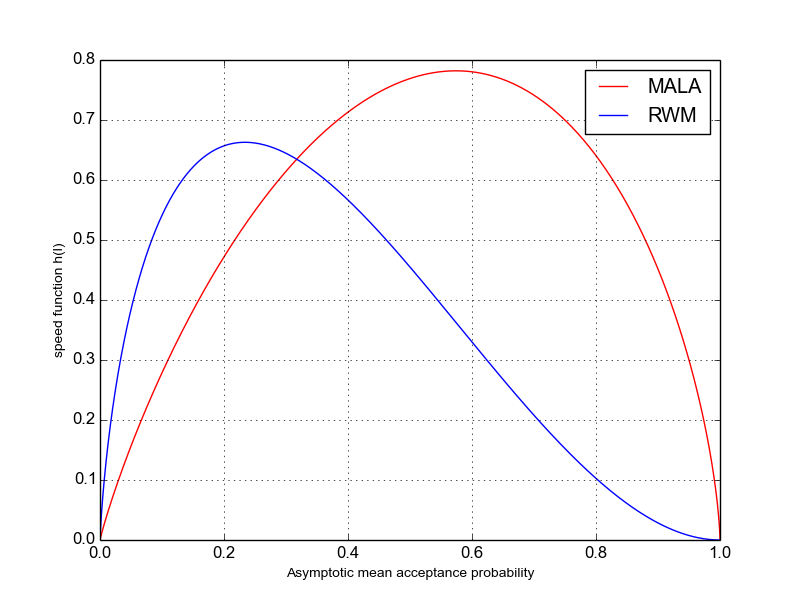
\includegraphics[width=0.75\textwidth]{speedmeasures}
 \end{center}
  \caption{Optimal acceptance probability for RWM=0.234 and MALA=0.574.}
  \label{fig:optimal acceptance probability}
\end{figure}

Through the convergence to an Gaussian random variable in Equation~(\ref{DLR-asymptotic mean acceptance probability}), the asymptotic mean acceptance probability~$\alpha^{\cdot}(l)$ can be explicitely computed and represented with the help of the culmulative density function~$\Phi$ of the standard normal distribution~\autocite[Lemma B2]{Beskos2009-2}. This convergence is also a crucial observation for later estimates. Generally speaking, the speed function varies the time-scale of the original diffusion given in Equation~(\ref{DLR-limit diffusion candidate}) by a factor~$h^{\cdot}(l)$ such that the effective time-step is reduced to $h^{\cdot}(l)\,t$ instead of $t$ as $ 0 \leq h^{\cdot}(l) \leq 1$. This results suggests choosing the value of~$l$ that maximizes the speed function~$h^{\cdot}(\cdot)$ since the limit diffusion~$z(t)$ will then explore the invariant measure as fast as possible. Obviously, the RWM and MALA algorithm have two different speed functions as the Gaussian random variables in Equation~(\ref{DLR-Gaussian RWM short}) and~(\ref{DLR-Gaussian MALA short}) distinguish. For practitioners, who often tune algorithms according to the acceptance probability of the simulation, it is relevant to express the maximization principle in terms of the asymptotic mean acceptance probability~$\alpha^{\cdot}(l)$. Figure~\ref{fig:optimal acceptance probability} shows that the speed function of the limit diffusion~$z(t)$ is maximized for an optimal asymptotic acceptance probability of $\alpha^{RWM}=0.234$ and $\alpha^{MALA}=0.574$, up to three decimal places. This fact is not surprisingly, as repeatedly stated, the MALA algorithm uses gradient information on the target measure. Note that this result extend the rules for an optimal tuning of Metropolis-Hastings methods from product target measures as seen in~\autocite{Bedard2007, Roberts1997, Roberts1998} to this class of non-product measures. For further details on this type of argument for RWM and MALA, we refer to the original papers~\autocite[Section 2.3, Section 2.6]{Mattingly2010, Pillai2012}, where the idea of this presentation is taken from.

Beside this convenient rule of thumb for the optimal tuning of the two MH methods, Theorem~\ref{DLR-THM main theorem} demonstrates that, in stationarity, the computional complexity to explore the invariant measure~$\pi$ scales as~$\mathcal{O}(N^{\gamma})$, where $\gamma=1$ for the RWM and $\gamma=1/3$ for the MALA, respectively. Indeed, we accelerated the interpolant~$z^N(t)$ in Equation~(\ref{DLR-linear continuous interpolant short}) by a factor~$(\Delta t)^{-1} = N^{\gamma}$ in order to observe a diffusion limit. This shows that $\mathcal{O}(N^{\gamma})$ steps of the Markov chain~$x^N$ as defined in Equation~(\ref{DLR-MH chain from algorithm - general form}) are required for $z^N(t)$ to approximate the diffusion process $z(t)$ on a time interval~$[0,T]$. This shows impressively the idea of the diffusion limit approach to measure the computational complexity of Metropolis-Hastings methods. As the argumentation is in some sense reversely, we will recall it. Since we know that the diffusion~$z(t)$ explores its invariant measure~$\pi$, and we have to accelerate the interpolant~$z^N(t)$ of the Markov chain~$x^N$ by a factor~$N^{\gamma}$ such that $z^N(t)$ converges to $z(t)$, hence $\mathcal{O}(N^{\gamma})$ steps of the chain~$x^N$ are required to explore the measure~$\pi$.


\section{Proof of main theorem}
\label{sec:DLR-Proof}

In order to prove Theorem~\ref{DLR-THM main theorem} we outline the proof strategy in Section~\ref{sec:sub:DLR-Proof strategy} and introduce the discrete drift-martingale decomposition of the Metropolis-Hastings~(MH) Markov chain. This decomposition is used to show (weak) convergence of the interpolant towards the drift and the noise term of the diffusion process given in Theorem~\ref{DLR-THM main theorem} by Equation~(\ref{DLR-Thm diffusion process}). Section~\ref{sec:sub:DLR-General diffusion approximation} states and proves a general diffusion approximation for Markov chains which satisfy an appropriate drift-martingale decomposition. In Section~\ref{sec:DLR-Proof}, we finally prove Theorem~\ref{DLR-THM main theorem} by pointing to key estimates in Section~\ref{sec:DLR-Estimates}, which will show that the decomposition of the MH chain given by Equation~(\ref{DLR-MH chain from algorithm - general form}) is appropriate.

\subsection{Proof Strategy}
\label{sec:sub:DLR-Proof strategy}


The main idea for the proof of Theorem~\ref{DLR-THM main theorem} is taken from numerical analysis. In fact, we will show that the Metropolis-Hastings Markov chain~$x^N$ generated by the RWM or MALA algorithm resembles a traditional Euler-Maruyama approximation scheme of the diffusion~$z(t)$ given by
 \begin{equation}
 \label{DLR-Proof: Definiton: diffusion process}
  dz = -h^{\cdot}(l) (z + \mathcal{C}_s \nabla \Psi(z)) dt + \sqrt{2 h^{\cdot}(l)} d\mathcal{W}(t),
 \end{equation}
where $h^{\cdot}(l) > 0$ and $\mathcal{W}(t)$ is a $\mathcal{C}_s$-Wiener process on $\mathcal{H}^s$. This is the diffusion limit in Theorem~\ref{DLR-THM main theorem}. To illustrate the idea of the proof of the theorem, we will give a short heuristical digression on approximations schemes for stochastic differential equations~(SDEs). The Euler-Maruyama scheme for the SDE in Equation~(\ref{DLR- diffusion process}) has the form for $0 \leq k \leq n-1$
\begin{equation}
\label{DLR-Proof: Definition Euler-Maruyama scheme of limit SDE}
\begin{split}
  Y_{k+1} & := Y_k - h^{\cdot}(l) (Y_k + \mathcal{C}_s \nabla \Psi(Y_k)) (t_{k+1} - t_k) + \sqrt{2 h^{\cdot}(l)} (\mathcal{W}(t_{k+1}) - \mathcal{W}({t_k})) \\
  & \; = Y_k + h^{\cdot}(l) \mu(Y_k) \Delta t + \sqrt{2 h^{\cdot}(l) \Delta t} \; Z_k,
\end{split}
\end{equation}
with initial condition~$Y_0 := x^{0,N}$ and the drift~$\mu: \mathcal{H}^s \to \mathcal{H}^s$ as defined in Equation~(\ref{DLR-Setting: Definition drift mu}) for an equidistant partition~$t_0 =0 < t_1 < \dots < t_{n-1} < t_n = T $ of~$[0,T]$ with $\Delta t := t_{k+1} - t_k$ and $Z_k \stackrel{D}{\sim} \mathcal{N}(0, \mathcal{C}_s)$. In the second identity, we used the fact, that $\mathcal{W}(t)$ is a $\mathcal{C}_s$-Wiener process, hence the increments are independently Gaussian distributed. Note that one may see $\mathcal{W}(t)$ equivalently as a Brownian motion on $\mathcal{H}^s$ with covariance operator~$\mathcal{C}_s$. These two notations describe the same object. Taking now the same interpolant as for the MH Markov chain as described in Equation~(\ref{DLR-linear continuous interpolant short}), we get the following rekursive expression for the Euler-Maruyama discretization~$Y(t)$ of the diffusion~$z(t)$ in the interval~$[0,T]$ for $t \in [k \Delta t, (k+1) \Delta t)$
\begin{align}
    Y(t) & \; = Y_k + \frac{t - k \Delta t}{\Delta t} (Y_{k+1} - Y_k) \nonumber  \\
    & \; = Y_k + \frac{t - k \Delta t}{\Delta t} (h^{\cdot}(l) \Delta t \, \mu(Y_k) +\sqrt{2h^{\cdot}(l) \Delta t } \; Z_k ) \nonumber \\
    & \quad \vdots \nonumber \\
    & \; = Y_0 + h^{\cdot}(l) \left[ \Delta t \sum_{i=0}^{k-1} \mu(Y_i) + (t - \Delta t) \mu(Y_k) \right] \label{DLR-Proof: Integralapproximation mu} \\ 
    & \qquad + \sqrt{2 h^{\cdot}(l)} \left\{ \sqrt{ \Delta t} \sum_{i=0}^{k-1} Z_i +  \frac{t - \Delta t}{\sqrt{\Delta t}} Z_k \right\} \label{DLR-Proof: Wiener process approximation}
\end{align}
Following the methodology of stochastic approximations schemes, we have to prove convergence of the quantity in the angular brackets in Equation~(\ref{DLR-Proof: Integralapproximation mu}) to the drift integral~$\int_0^t \mu (t) dt$ of the original SDE and we have to show an \textit{invariance principle}, in the sense of a generalization of Donsker's Theorem as in~\autocite{Revuz2005}, for the quantity in the curly brackets in Equation~(\ref{DLR-Proof: Wiener process approximation}). Such an invariance principle states  that a rescaled sum of random variables, as the quantity in the curly brackets, converges weakly to a Wiener process~$\mathcal{W}(t)$ on $\mathcal{H}^s$ with a covariance operator~$\mathcal{C}_s$. 
\newline


Keeping this in mind, let $\mathcal{F}_k$ denote the sigma algebra generated by~$\{ x^{i,N}, \xi^{i,N}, \gamma^{i,N} : i \leq k  \}$. We denote the conditional expectation by~$\mathbb{E}[|\mathcal{F}_k]$. We define now the \textit{drift-martingale decomposition} of the Metropolis-Hastings chain~$x^N = \{ x^{k,N} \}_{k \geq 0}$ by introducing the drift function~$d^N: \mathcal{H}^s \to \mathcal{H}^s$ given by
\begin{equation}
\label{DLR-Proof: Definition drift function d^N}
d^N (x) := \left(  h^{\cdot}(l) \Delta t \right)^{-1} \mathbb{E} \left[ x^{1,N} - x^{0,N} | x^{0,N} = x \right] 
\end{equation}
and the martingale difference array~$\{ \Gamma^{k,N} (x^{k,N}, \xi^{k,N})= \Gamma^{k,N} : k \geq 0 \}$ defined by
\begin{equation}
 \label{DLR-Proof: Definiton martingale difference array}
 \Gamma^{k,N} := \left( 2 h^{\cdot}(l) \Delta t \right)^{-1/2} \left( x^{k+1,N} -x^{k,N} - h^{\cdot}(l) \Delta t d^N (x^{k,N})  \right).
\end{equation}
For the drift-martingale decomposition the natural time step is given by $\Delta t := N^{-\gamma}$ as in Theorem~\ref{DLR-THM main theorem}. By definition, $\Gamma^{k,N}$ is a $\mathcal{F}_k$-martingale for any~$N\geq1$. The drift-martingale decomposition of the Markov chain~$\{ x^{k,N} \}_{k}$ then reads
\begin{equation}
 \label{DLR-Proof: Definition drift-martingale decomposition}
 x^{k+1,N} - x^{k,N} = h^{\cdot}(l) \Delta t \, d^N(x^{k,N}) + \sqrt{2 h^{\cdot}(l) \Delta t} \, \Gamma^{k,N}.
\end{equation}
This identitiy follows directly by inserting the definition of the drift martingale array. According to the methodology of numerical analysis, we now interpolate our time-discrete chain continuously and piecewise linearly as defined in Equation~(\ref{DLR-linear continuous interpolant short}) and used in the heuristic digression. Thus the interpolant~$z^N(t)$, $t \in [0,T]$, has the form 
\begin{align}
  z^N(t) & \; = x^{0,N} + h^{\cdot}(l) \left[ \Delta t \sum_{i=0}^{k-1} d^N(x^{i,N}) + (t - \Delta t) d^N(x^{k,N}) \right] \label{DLR-Proof: Integralapproximation d^N} \\ 
  & \qquad + \sqrt{2 h^{\cdot}(l)} \left\{ \sqrt{ \Delta t} \sum_{i=0}^{k-1} \Gamma^{i,N} +  \frac{t - \Delta t}{\sqrt{\Delta t}} \Gamma^{k,N} \right\} \label{DLR-Proof: Gamma approximation}
\end{align}
for $k \Delta t \leq t  < (k+1) \Delta t $ and $\Delta t = N^{-\gamma}$. In order to show now weak convergence in $C([0,T];\mathcal{H}^s)$ of the interpolant~$z^N(t)$ to the diffusion~$z(t)$ given in Equation~(\ref{DLR-Proof: Definiton: diffusion process}), one has to verify that the quantity in the angular brackets in Equation~(\ref{DLR-Proof: Integralapproximation d^N}) converges to the drift of $z(t)$ and the quantity in the curly brackets in Equation~(\ref{DLR-Proof: Gamma approximation}) converges to a $\mathcal{C}_s$-Wiener process in $\mathcal{H}^s$, i.e.,
\begin{equation}
  \begin{split}
   \Delta t \sum_{i=0}^{k-1} d^N(x^{i,N}) + (t - \Delta t) d^N(x^{k,N}) \Longrightarrow \int_0^t \mu(z(t)) dt, \\
   W^N(t) := \sqrt{ \Delta t} \sum_{i=0}^{k-1} \Gamma^{i,N} +  \frac{t - \Delta t}{\sqrt{\Delta t}} \Gamma^{k,N} \Longrightarrow \mathcal{W}(t), \\
 \end{split}
\end{equation}
where $\Longrightarrow$ denotes weak convergence in $C([0,T];\mathcal{H}^s)$ for $N \to \infty$ and $\mathcal{W}(t)$ denotes a Wiener process on $\mathcal{H}^s$ with  covariance operator~$\mathcal{C}_s$. A key point for the convergence of the drift term is the fact that quantity~$Q^N_{\cdot}(x, \xi^N)$ has a Gaussian behavior for large~$N$ such that one can give a quantitative version of the approximation~$ d^N(x) \approx \mu(x) $, see Lemma~\ref{}. To prove the convergence of the \textit{noise}~$W^N(t) \in C([0,T];\mathcal{H}^s)$, we establish an invariance principle for the rescaled version of the martingale difference array given by $W^N(t)$. Indeed, Proposition~\ref{} proves the stronger result
\begin{equation*}
  (x^{0,N}, W^N) \Longrightarrow (z^0, \mathcal{W}),
\end{equation*}
where $\Longrightarrow$ denotes weak convergence in $\mathcal{H}^s \times C([0,T];\mathcal{H}^s)$, and $z^0 \stackrel{D}{\sim} \pi$ is independent of the limiting Wiener process~$\mathcal{W}(t)$. Using this invariance principle for~$W^N$ and the fact of additive noise in the diffusion limit~$z(t)$, we deduce the weak convergence of~$z^N$ to $z$ in $ C([0,T];\mathcal{H}^s)$ from a continuous  mapping argument (It\={o} map), see Proposition~\ref{}. This continuous mapping argument, which we will now outline, allows us to manage the transfer from the drift term with $d^N(x)$ given in Equation~(\ref{DLR-Proof: Integralapproximation d^N}) to the desired drift~$ \int_0^t \mu(z) du$ of the limiting SPDE given in Equation~(\ref{DLR-Proof: Definiton: diffusion process}). 

Define the It\={o} map~$\Theta$ for any $\omega \in C([0,T];\mathcal{H}^s)$ by 
\begin{equation*}
 \Theta : \mathcal{H}^s \times C([0,T];\mathcal{H}^s) \to C([0,T];\mathcal{H}^s)
\end{equation*}
which maps~$(z^0, \omega)$ to the unique solution of the integral equation
\begin{equation}
  z(t) := z^0 - h^{\cdot}(l) \int_0^t \mu(z) du + \sqrt{2 h^{\cdot}(l)} \omega(t) \qquad \forall t \in [0,T].
\end{equation}
Note that $z := \Theta (z^0, \mathcal{W})$ solves the limiting SPDE given in Theorem~\ref{DLR-Thm diffusion process}:
\begin{equation}
 z(t) = z^0 -  h^{\cdot}(l) \int_0^t (z(u) + \mathcal{C}_s \nabla \Psi(z(u))) du + \sqrt{2 h^{\cdot}(l)} \mathcal{W}(t) \qquad \forall t \in [0,T],
\end{equation}
where~$\mathcal{W}(t)$ is a $ \mathcal{H}^s $-valued  $ \mathcal{C}_s $-Wiener process.













Before we put the proof into action, we want to emphasize arising difficulties.



\subsection{General Diffusion Approximation}
\label{sec:sub:DLR-General diffusion approximation}

\subsection{Proof of Theorem~\ref{DLR-THM main theorem}}
\label{sec:sub:DLR-Proof}

\section{Key Estimates}
\label{sec:DLR-Estimates}

\subsection{Technical Lemmas}

\subsection{Gaussian Approximation}

\subsection{Drift Approximation}

\subsection{Noise Approximation}
 
\subsubsection{Martingale Invariance Principle}
\label{Martingale invariance principle}

This section proves that the process $ W^{N} $ defined in Equation~?? converges to an appropriate Wiener process.

\begin{proposition}
 \label{Invariance principle}
 Let Assumption~?? hold. Let $ z^0 \stackrel{D}{\thicksim} \pi $ and $ W^{N}(t) $, the process defined in Equation~??, and $ x^{0,N} \stackrel{D}{\thicksim} \pi^{N} $, the starting position of the Markov chain $ x^{N} $, defined in Equation~??. Then
 \begin{equation}
  (x^{0,N}, W^{N}) \Longrightarrow (z^0, \mathcal{W}),
 \end{equation}
 where $ \Longrightarrow $ denotes weak convergence in $ \mathcal{H}^s \times C \left( [0,T]; \mathcal{H}^s \right) $, and $ \mathcal{W}$ is a $ \mathcal{H}^s $-valued  $ \mathcal{C}_s $-Wiener process. Furthermore the limiting Wiener process~$ \mathcal{W} $ is independent of the initial condition $ z^0 $.
 
\end{proposition}



We will use the following result concerning triangular martingale increment arrays taken from~\autocite{Berger1986}. The result is similar to the classiscal results on triangular arrays of independent increments and is generally spoken a generalization of a martingale central limit theorem.

Let $ k_{N}: [0,T] \to \mathbb{Z}_{+} $ be a sequence of nondecreasing, right-continuous functions indexed by $ N $ with $ k_{N}(0) = 0 $ and  $k_{N} (T) \geq 1 $. Let $ \{ M^{k,N}, \mathcal{F}^{k,N}  \}_{0 \leq k \leq k_{N}(T)} $ be an $ \mathcal{H}^s $-valued martingale difference array. That is, for $ k = 1,\dots , k_{N}(T) $, we have
$  \mathbb{E} \left[  M^{k,N} | \mathcal{F}^{k-1,N} \right] =  0 $,  $  \mathbb{E} \left[ \| M^{k,N} \|_{s}^{2} \; | \mathcal{F}^{k-1,N} \right] <  \infty $ almost surely
and $ \mathcal{F}^{k-1,N} \subset \mathcal{F}^{k,N} $.

\begin{proposition}\autocite[Theorem 5.1]{Berger1986}
\label{Martingale central limit theorem - Helping proposition}
  Let $ S : \mathcal{H}^s \to \mathcal{H}^s $ be a self-adjoint, positive definite operator with finite trace. Assume that, for all $ x \in \mathcal{H}^s $, $ \varepsilon > 0 $ and $ t \in [0,T] $, the following limits hold in probabiity:
  \begin{align}
   \lim_{N \to \infty} \sum_{k=1}^{k_{N}(T)} \mathbb{E} &\left[ \| M^{k,N} \|_{s}^{2}  \; | \mathcal{F}^{k-1,N} \right] = T \; \text{Tr}_{\mathcal{H}^s}(S), \label{MCLT - P1}\\
   \lim_{N \to \infty} \sum_{k=1}^{k_{N}(t)} \mathbb{E} &\left[ \langle  M^{k,N} , x \rangle_{s}^{2}  \; | \mathcal{F}^{k-1,N} \right] = \langle Sx , x \rangle_{s}, \label{MCLT - P2}\\
   \lim_{N \to \infty} \sum_{k=1}^{k_{N}(T)} \mathbb{E} &\left[ \langle M^{k,N} , x \rangle_{s}^{2} \; 1_{\{ | \langle M^{k,N} , x \rangle_s \; | \leq \varepsilon \}} | \mathcal{F}^{k-1,N} \right] = 0. \label{MCLT - P3}
  \end{align}
  Define a continuous time process $ W^{N} $ by $ W^{N}(t) := \sum_{k=1}^{k_{N}(t)} M^{k,N} $ if $ k_{N}(T) \leq 1 $ and $ k_{N}(t) > \lim_{r \to 0_+} k_N(t-r) $, and by linear interpolation otherwise.
  
  Then the sequence of random variables $ W^N $ converges weakly in $ C \left( [0,T]; \mathcal{H}^s \right) $ to an $ \mathcal{H}^s $-valued $S$-Wiener process $\mathcal{W}(t)$, with $ \mathcal{W}(0) = 0 $, $ \mathbb{E} [ \mathcal{W}(T) ] =  0 $.
  
\end{proposition}

\begin{rem}
The first two hypotheses of the above proposition ensure the weak convergence of finite-dimensional distributions of $ W^{N}(t) $ using the martingale central limit theorem in $ \mathbb{R}^N $. The last hypothesis, the conditional Lindeberg assumption, is needed to conclude the tightness of the famili $ \{ W^{N}(\cdot) \}  $. As noted in~\autocite{ChenWhite1998}, the hypothesis (\ref{MCLT - P2}) can be replaced by
 \begin{equation}
  \lim_{N \to \infty} \sum_{k=1}^{k_{N}(t)} \mathbb{E} \left[ \langle  M^{k,N} , e_n \rangle_{s} \langle  M^{k,N} , e_m \rangle_{s} \; | \mathcal{F}^{k-1,N} \right] = \langle Se_n , e_m \rangle_{s}, \label{MCLT - P2 - new}
 \end{equation}
 in probabiity, where $ \{ e_m \}_{m} $ is any orthonormal basis for $ \mathcal{H}^s $. The Lindeberg type condition (\ref{MCLT - P3}) is implied by
 \begin{equation}
  \lim_{N \to \infty} \sum_{k=1}^{k_{N}(T)} \mathbb{E} \left[ \| M^{k,N} , x \|_{s}^{2} \;  1_{\{ \| M^{k,N} \|_{s}^{2} \; | \leq \varepsilon \}} | \mathcal{F}^{k-1,N} \right] = 0. \label{MCLT - P3 - new}
 \end{equation}
 in probabiity, for any fixed $ \varepsilon > 0 $.

\end{rem}

\begin{proof}(of the invariance principle)
 Applying Proposition~\ref{Martingale central limit theorem - Helping proposition}, we define the following quantities $ k_N(t) := \lfloor Nt \rfloor $, $ M^{k,N} := \frac{1}{\sqrt{N}} \Gamma^{k,N} $ and $ S := \mathcal{C}_s $.  The resulting definition of $ W^{N}(t) $ from Proposition~\ref{Martingale central limit theorem - Helping proposition} coincides with that given in (?REF NEEDED!) as we used a continuous, linear interpolation.
\end{proof}

